\section{as Model Classes}

To a deity with unbounded computational powers, all that can be known about an object $x$ can be conveyed in $\KC(x)$ bits.
In that sense, Kolmogorov complexity is a measure of the information in an object.
In practice, however, part of the information thus measured may be out of reach.
Next to computational reasons, this may be because of the expectations an observer has about an object.
As an observer may not be receptive to all information, it may be possible to convey a sufficient part of the information in an object $x$ in under $\KC(x)$ bits.
This is what lossy compression aims for.

\begin{example}
\label{ex:useful_information}%
  \indexkey{example!image compression}%
  To get a feel for the amount of information in an object that is relevant, we take a brief look at image compression.
  The Kolmogorov complexity of an image can be approximated from above using a lossless graphics file format such as Portable Network Graphics, PNG~\parencite{sayood2017introduction}.
  In turn, the information that is actually observed can be approximated using a lossy file format such as JPEG~\parencite{sayood2017introduction}.
  Looking at the Kodak True Color Image Suite \parencite{franzen1999kodak}, a standard test set, we find the following mean file sizes \parencite{sneyers2016flif}.
  \begin{center}
    \begin{tabular}{cc}
    \emph{PNG}	& \emph{JPEG~(Q=90)} \\
    \hline
	%641429 byte	& 135557 byte \parencite{sneyers2016flif}, 135805 byte (experimental)
    641~kilobyte	& 136~kilobyte
    \end{tabular}
  \end{center}
  This puts the fraction of the information in an image that is essential to it's qualities as an image at around $21\%$.
\end{example}

In the presentation of an object, a certain amount of redundancy is desirable.
Hardly ever do we want an object to be displayed as a string witnessing just its useful information, or even its Kolmogorov complexity.
When we derive a length notion from a more natural presentation, this length can be divided into three parts.
These parts are: the \emph{useful information}, the \emph{noise}, and the \emph{redundancy}, as shown in Figure~\ref{fig:length_decomposed} on page~\pageref{fig:length_decomposed}.
Here, noise is the difference between the Kolmogorov complexity and the useful information.

\begin{example}[continued]
\label{ex:bmp_png_jpeg}%
  \indexkey{example!image compression}%
  The most natural presentation of an image is as its intended graphical display.
  Via the bitmap image file format, BMP, we get a length measure that is, at least in spirit, derived from this means of presentation.
  The images in the Kodak image suite all contain $768 \cdot 512 = 393216$ pixels, each recorded with $3$ bytes of color depth.
  Thus, the BMP size of each image is 1180~kilobyte.
  In relation to this, the images contain, on average, at most $11\%$ useful information, around $43\%$ noise, and at least $46\%$ redundant information.
\end{example}

That not all of some object's natural length is allotted to useful information can also be seen from information hiding techniques.
Homoglyphs are text characters that are not perceived to be different, yet have different encodings.
By selectively replacing characters in a text message by their homoglyphs, information can be injected into a message without ostensibly altering it.
Arguably, the information in a text message is not even altered when words or phrases in it are replaced by synonyms.
This, too, can be used for information hiding, or, more technically, for \defkey{steganography} \parencite{hosmani2015dual}.

While the useful information is left unaltered by steganography, this does not mean that the presence of hidden information cannot be detected.
Such detection is the goal of \emph{steganalysis}.
For instance, it is not unreasonable to expect that the use of homoglyphs reduces the redundancy in a message.
Thus, a carrier message \emph{without} hidden information may be more compressible than a message \emph{with} hidden information.
Applied to images, techniques are developed to restrict the action of steganographic information hiding to the noise in an image.
These techniques evade detection by simple compression tests.
An overview of steganography methods for images is given by \textcite{cheddad2010digital}.

The traditional formalization of useful information, \emph{sophistication}, targets a universal observer with unbounded computational powers.
This approach is complicated by the fact that, unlike Kolmogorov complexity, sophistication differs without bounds among universal observers.
Additionally, if we consider reasoning to be a form of computation, then it makes sense to include computational complexity in a measure of useful information.
With parameterizations, we can formalize useful information in a context-sensitive way.
Moreover, since parameter values can provide a measure of computational complexity, a parameterized sophistication can include computational considerations.
Doing so tightens the relationship between algorithmic complexity and computational complexity.

\subsubsection{Synopsis}
\todo[inline]{
  TODO

  NOTE: instances are string that result from encoding objects.

  NOTE: This entire section is about quasiparameterizations.

  In the section on Sophistication (at least), traditional algorithmic statistics is used as a running example of parameterized algorithmic statistics.

  Most definitions are straightforward generalizations of their traditional counterparts and many theorems resolve questions that are central to the traditional setting.

  The sections on stochasticity, estimators, and data structures investigate the existence and prevalence of strings (objects/events) without simple models.
}

\subsection{An Overview of Algorithmic Statistics}
The crucial insight that makes algorithmic statistics possible is that the Kolmogorov complexity of an object can always be realized by a two-part code.
Every object can be described by two strings of which the combined length equals, up to an independent additive constant, the Kolmogorov complexity of the object.
The two parts are commonly called \defkey{model} and \defkey{data-to-model code}.
The second part is so named because it describes the object relative to the model.
In the pairing of the two parts it must be clear where one part ends and the other begins.

In traditional applications of the minimum description length principle \parencite{rissanen1978modeling,rissanen1983universal,vitanyi2000minimum,grunwald2007minimum} the word `model' is used to indicate a functional form.
The second part of the two-part code is then used to both instantiate a single function \emph{and} specify the data with respect to it.
In algorithmic statistics, however, the two-part code should separate the meaningful information in an object from the random noise in that object.
Algorithmic statistics is not concerned with any structure inside the second part of the two-part code.
Thus, the word `model' is used for what is known as a \emph{point hypothesis} or \emph{exact hypothesis} in inferential statistics.
More concretely, in algorithmic statistics, we interpret models as probability distributions.
In turn, data-to-model codes are interpreted as entropy encodings in accordance with those probability distributions \parencite{vereshchagin2004kolmogorov,cover2006elements}.

A measure of the informativeness, the \defkey{sophistication}, of an object is available in the form of the minimum complexity of a model for the object.
This minimization is restricted to those probability distributions with which the two-part code for the object realizes the Kolmogorov complexity of the object.
Unfortunately, there is no clear-cut way to define the complexity of a probability distribution.
If we would allow the universal distribution \parencite{li2008introduction} to have a finite complexity, then it would realize the Kolmogorov complexity of every object.
In that sense, it would act as a universal model \parencite{vitanyi2006meaningful,bloem2015two}.
Disregarding additive constants for a moment, we see that such a universal model would place a universal bound on the informativeness of any object.
This renders our measure of informativeness useless.
To which probability distributions we assign finite complexity is hence a central question in the development of algorithmic statistics \parencite{vereshchagin2017algorithmic}.
The class of probability distributions considered is called the \emph{model class}.
While the choice of a model class is usually an ad~hoc choice in applications of the minimum description length principle \parencite{vitanyi2000minimum,grunwald2007minimum}, algorithmic statistics calls for a single generic model class.
The lack of a universally best model class, according to some motivation from outside the theory, is a major obstacle for algorithmic statistics.

Many model classes have been considered in the existing literature.
When interpreted as classes of probability distributions, there is significant variation in the requirements that have been put on the computability of the probabilities.
Regardless of this variation, the studied model classes can be characterized by a classification of the \emph{support} of the probability distributions they contain.
Least restrictive are the model classes where the support of a probability distributions can be any semidecidable set.
Such model classes are present in the works of \textcite{rissanen1983universal}, \textcite{koppel1988structure}, \textcite{gacs2001algorithmic} (as implicit probabilistic models), \textcite{vitanyi2006meaningful}, and \textcite{antunes2009sophistication}.
A model class where exactly the decidable sets occur as the support of the probability distributions is hinted at by \textcite{gacs2001algorithmic} (as explicit probabilistic models).
However, their definitions are not strong enough to enforce decidability.
The most fruitful model class has been that of uniform probability distributions with arbitrary, yet necessarily finite, support.
This is the model class originally proposed by Kolmogorov and most prominent in the works of \textcite{gacs2001algorithmic,vereshchagin2004kolmogorov}.
A slightly more general model class where the probability distributions have finite support, yet are allowed to take on different rational-valued probabilities on their support, was considered by \textcite{vereshchagin2017algorithmic}.

All of the model classes studied by the aforementioned authors exclude universal models.
Yet, none are presented with a guarantee against putting meaningful information in the data-to-model code, thus \emph{underfitting} the data.
As argued by \textcite{bloem2015two}, it is likely that these model classes do in fact contain models that are `too universal'.
That is, some models are universal enough to bound the informativeness of objects that we think of as containing meaningful information.
At the same time, \textcite{bloem2015two,antunes2017sophistication} show that the choice of the complexity measure used to measure the complexity of models matters.
Sophistication, which is described in more detail in the next section, in particular is sensitive to this choice.
While Kolmogorov complexity is invariant under the choice of a universal machine, sophistication, despite being based on Kolmogorov complexity, is not.
This is true regardless of which of the many ways \parencite{gacs2001algorithmic} we pick to adapt Kolmogorov complexity for measuring the complexity of probability distributions.
Slight variations in the model complexity can change a model from realizing the Kolmogorov complexity of an object to not realizing it and vice versa.
Hence the minimum complexity of a probability distribution with which the two-part description of an object realizes the Kolmogorov complexity of that object can change significantly with a change of the reference universal machine.
As a result, some choices of a reference machine may lead to widespread \emph{overfitting} \parencite{bloem2015two}.
When performing maximum likelihood estimation, this form of overfitting can be mitigated by working with complexity-constrained subclasses of the model class \parencite{vereshchagin2004kolmogorov}.
However, that brings us no closer to a definitive measure of the useful information in an object.
Alternatively, one can adjust the complexity measure for models so that the selection of overfitting models is penalized.
This is done by \textcite{rissanen1983universal,antunes2009sophistication}, but it is not proven to be effective and may lead to underfitting instead \parencite{bloem2015two}.

We propose to include the model class and its associated complexity measure as a variable in the framework of algorithmic statistics.
Besides addressing underfitting and overfitting, doing so also makes it possible to examine complexity measures other than the Kolmogorov complexity.
The uncomputability of Kolmogorov complexity has been identified as an impediment to applications of algorithmic statistics \parencite{rissanen1983universal,vereshchagin2017algorithmic}.
Remarkably, the existing literature on algorithmic statistics has so far only considered variations of Kolmogorov complexity as complexity measures.
By contrast, the potential for restricted model classes has been identified \parencite{bloem2014safe,vereshchagin2017algorithmic}.
By introducing an explicit dependence on a model class, we accept that a notion of useful information may be subject to one's inclination.
There appears to be no universally best model class, or, in other words, no universal prior for algorithmic statistics.
Because of that, the dependence of a notion of useful information on a model class is likely unavoidable.
\slogan[\label{slo:useful_information}]{Useful information is context-dependent.}
Accepting that a notion of useful information is dependent on a model class justifies the addition of a model class variable to the framework.

\subsection{Sophistication}
Traditionally, algorithmic statistics looks at describing a string $x$ with the help of a probability distribution $P$ that assigns nonzero probability to $x$.
The probability mass function $P$ is required, at the least, to be rational-valued and computable \parencite{vereshchagin2017algorithmic}.
Knowing $P$, a code that is optimal with respect to $P$ needs $-\log P(x)$ bits for describing $x$ in prefix-free fashion \parencite{cover2006elements}.
Now, let us use $\length{P}$ for the length of a description of $P$ in some fixed prefix-free encoding of rational-valued computable probability mass functions.
We find an upper bound on the Kolmogorov complexity of $x$ in the form of a two-part description of $x$,
\begin{equation*}
  \KC(x) \le \length{P} - \log P(x).
\end{equation*}
How tight this bound can get depends on the chosen method of encoding probability mass functions.
It is customary to focus on methods that are as efficient as possible.
When the support of a distribution $P$ is a singleton $\{x\}$, its length $\length{P}$ can be made to match, up to an additive constant, the Kolmogorov complexity of $x$.
For such encodings, the above equation can become an equality.

Since we are describing the string $x$ using two-part codes, we may investigate the many ways in which a description of $x$ can be composed of two parts.
In particular, we are interested in the ways the Kolmogorov complexity of $x$ can be split in two by probability mass functions.
Naturally, when we restrict our model class, we limit the number of ways to describe $x$.
However, some model classes nearly cover all possible ways to balance the lengths of the two parts.
One such model class is that of uniform distributions.
The support of a uniform probability mass function is a finite set.
For a finite set $A$, let $\langle A\rangle$ denote a listing of all elements of $A$ and notice that the number of elements of $A$ can be recovered from~$\langle A\rangle$.
\begin{theorem}[{\textcite[Remark~1 \& Proposition~6]{vereshchagin2017algorithmic}}]\hspace{0pt}\\*
\label{thm:uniformmodels}%
  Let $P$ be a rational-valued computable probability mass function and $x$ a string to which $P$ assigns nonzero probability.
  There exists a finite set $A$ of $m$ elements including $x$ such that we have
  \begin{equation*}
    \KC(\langle A\rangle) \le \length{P} + \bigO(\log \length{x}) \quad\text{and}\quad -\log \frac{1}{m} \le -\log P(x) + \bigO(1).
  \end{equation*}
\end{theorem}
In other words, up to terms logarithmic in the length of a string $x$, we may restrict our attention to uniform distributions.
Uniform distributions effectively maximize the minimum probability in a distribution with a given finite support.
For distributions with a given infinite support, there is no clear-cut way of maximizing the minimum probability.
Therefore, it is interesting to note that there is a variant of Theorem~\ref{thm:uniformmodels} for a model class where distributions have potentially infinite support.
Note that the $-\log \frac{1}{m}$ term in Theorem~\ref{thm:uniformmodels} represents the fact that $\log m$ bits suffice to tell the elements of the finite set $A$ apart.
With Elias~delta coding\indexkey{Elias~delta coding}, we can single out the $r$th element of any decidable set using $2 \log \log r + \log r$ bits.
Prefix-free codes such as the Elias~delta coding are related to probability distributions by the \defkey{Kraft~inequality} \parencite{cover2006elements,li2008introduction}.
An element that is encoded using $\ell$ bits is accordingly assigned a probability of $2^{-\ell}$.
The probability distributions stemming from Elias~delta coding via the Kraft~inequality can have infinite support.
It is the model class of such distributions that has a property similar to that codified in Theorem~\ref{thm:uniformmodels} for the model class of uniform distributions.
For a decidable set $A$, let $\KC(A)$ denote the least length among the lengths of decision procedures for $A$.
\begin{theorem}
\label{thm:rankmodels}%
  Let $P$ be a rational-valued computable probability mass function and $x$ a string to which $P$ assigns nonzero probability.
  There exists a decidable set $A$ including $x$ such that, with $r \deq \rank(x : A)$, we have
  \begin{align*}
    \KC(A) &\le \length{P} + \bigO(\log \length{x})
  \shortintertext{and}
    2 \log \log r + \log r &\le -\log P(x) + \bigO(1).
  \end{align*}
\end{theorem}
\begin{proof}
  Let $S$ be the support of $P$ and let $r_S$ be the rank of $x$ in this set.
  In other words, we define $S$ as $\{y \st P(y) > 0\}$ and we define $r_S$ as $\rank(x : S)$.
  Furthermore, set $i$ to the unique value for which we have
  \begin{equation*}
    \frac{i^2\, 2^i}{(\log r_S)^2\, r_S} < P(x) \le \frac{(i + 1)^2\, 2^{i + 1}}{(\log r_S)^2\, r_S}.
  \end{equation*}
  Observe that $i$ must be less than $\log r_S$, because $P(x)$ is at most $1$.
  Therefore, we have $i \in \bigO(\length{x})$ and the number of bits needed to specify $i$ is in $\bigO(\log \length{x})$.

  Now, consider the set
  \begin{equation*}
    H \deq \left\{y \st[\middle] P(y) > \frac{i^2\, 2^i}{(\log \rank(y : S))^2\, \rank(y : S)}\right\}.
  \end{equation*}
  We find that $x$ is included in $H$ and that the rank of $x$ in $H$ is at most
  \begin{equation}
  \label{eq:rankmodels:rank}
    \frac{(\log r_S)^2\, r_S}{i^2\, 2^i},
  \end{equation}
  for otherwise the sum of the probabilities would exceed $1$.
  To complete the proof, all that remains is to move some complexity from the data-to-model code into the model.
  The set $H$ can be partitioned into $\length{x}^2$ subsets $H_1, H_2, H_3, \ldots, H_{\length{x}^2}$ via
  \begin{equation*}
    H_j \deq \{y \in H \st \rank(y : H) \equiv j \pmod{\length{x}^2}\}.
  \end{equation*}
  For exactly one $j$, the set $H_j$ contains $x$.
  Let $A$ be this set $H_j$.
  That is, $A$ is a thinned out version of $H$ that includes $x$.
  By construction, $A$ contains only one out of every $\length{x}^2$ elements of $H$.
  Following \eqref{eq:rankmodels:rank}, the rank of $x$ in $A$ is therefore at most
  \begin{equation*}
    \frac{(\log r_S)^2\, r_S}{i^2\, 2^i} / \length{x}^2,
  \end{equation*}
  which is at most $\frac{r_S}{i^2\, 2^i}$.
  Thus, if we let $r$ denote this rank, we find
  \begin{align*}
    2 \log \log r + \log r &\le 2 \log \log \frac{r_S}{i^2\, 2^i} + \log \frac{r_S}{i^2\, 2^i} \\
    	&< 2 \log \log r_S + \log r_S - 2 \log i - i \\
    	&\le -\log \frac{(i + 1)^2\, 2^{i + 1}}{(\log r_S)^2\, r_S} + \bigO(1) \\
    	&\le -\log P(x) + \bigO(1),
  \end{align*}
  as desired.
  Additionally, $A$ was constructed from $P$, $i$, and $j$, so we also have $\KC(A) \le \length{P} + \bigO(\log \length{x})$.
\end{proof}

The message of Theorem~\ref{thm:rankmodels} is that, up to terms logarithmic in the length of a string $x$, we may restrict our attention to distributions in accordance with Elias~delta coding.
This allows us to focus on decidable sets as models, and on quasiparameterizations with decidable slices as model classes.
\begin{definition}
  A \defkeyat{parameterized!model}{parameterized model} is a slice of a quasiparameterization, represented by its corresponding parameter value.
\end{definition}

We call a quasiparameterization~$\eta$ a \defkeyat{parameterized!model class}{parameterized model class}, and a parameter value~$k$ an \emph{$\eta$"~model} for a string~$x$ if we have $x \in \eta_k$.
By using the same coding method for all slices, even for all quasiparameterizations, we are able to isolate the useful information about an object.
We are unable to express any properties about the rank of a string~$x$ in a slice~$\eta_k$ if our data-to-model code is confined to Elias~delta coding.
Therefore, useful information can only accumulate in a specification of the model, thus in the parameter value~$k$.

One way to think of a quasiparameterization in this context is as a sort of alternative computability universe.
In such an alternative universe, the slices of the quasiparameterization take the role of \enquote{decidable} sets.
Parameter values then encode the equivalent of the corresponding decision procedures.
Of course, when not all slices of the quasiparameterization are decidable, this alternative universe is different from the universe we inhabit.
However, even when all slices are decidable, the quasiparameterization may still challenge our notion of how computability behaves.
The parameter value associated with a slice may not be related to anything we would reasonable want to call a decision procedure for the slice.
On the other hand, when we can effectively map the parameter values to decision procedures for the respective slices, we are in a fairly restricted setting.
\begin{example}
  The quasiparameterization that best reflects our universe in terms of computability is given by
  \begin{equation}
  \label{eq:quasi_decision}
    (\{x \st \text{$k$ encodes a decision procedure that accepts $x$}\})_{k \in \binary^+}.
  \end{equation}
  In this quasiparameterization, there are two kinds slices.
  For a parameter value $k$ that encodes a decision procedure, the corresponding slice is the set decided by that decision procedure.
  However, if $k$ does not encode a decision procedure, for instance because $k$ does not encode a total function, the corresponding slice is empty.
  Unfortunately, by Rice's theorem \parencite{rice1953classes}, this means we cannot effectively map a parameter value to a decision procedure for the corresponding slice.
\end{example}

Suppose it is possible to map parameter values to decision procedures for the corresponding slices of a quasiparameterization effectively.
Then, the minimum length of a decision procedure for a slice is, up to an additive constant, bounded from above by the length of the corresponding parameter value.
The additive constant only depends on the algorithmic complexity of the function mapping parameter values to decision procedures.
Because this constant is fixed for the quasiparameterization, we may ignore it and use the length of a parameter value as the length of a decision procedure.
For more unusual quasiparameterizations such a constant may not exist.
Yet, we may still use the length of a parameter value as a measure of the complexity of a slice.
In general, a nice starting point for measuring the algorithmic complexity of a string with respect to a quasiparameterization is the following.
\begin{definition}
  The \defkeyat{parameterized!complexity}{parameterized complexity} of a string $x$ with respect to a quasiparameterization $\eta$ is
  \begin{equation*}
    \pc_\eta(x) \deq \min\{\length{\pair{k}{\rank(x : \eta_k)}} \st x \in \eta_k\}.
  \end{equation*}
\end{definition}
As quasiparameterizations are covers of $\binary^+$, the parameterized complexity with respect to a quasiparameterization is defined for every string.
Note that the choice of a pairing function may have an effect on the parameterized complexity.
It may effect not only its value, but also the parameter value with which this value, as a minimum of multiple candidates, is realized.

\begin{example}[continued]
\label{ex:traditional_pc}%
  So far, we have used a pairing function that concatenates the components of the pair after encoding them using a prefix-free code.
  When encoding procedures, however, it is natural to use a prefix-free code to begin with \parencite{li2008introduction}.
  Suppose we use such an encoding for the quasiparameterization given by~\eqref{eq:quasi_decision}.
  In that case, the parameter values of the subparameterization consisting of only the nonempty slices already form a prefix-free set.
  We can therefore consider the pairing function that concatenates the parameter value with the rank, after the latter is encoded using, say, Elias~delta coding.

  It turns out that parameterized complexity with respect to the quasiparameterization given by~\eqref{eq:quasi_decision} is essentially Kolmogorov complexity.
  To see that it is at most the Kolmogorov complexity, observe that for every string~$x$, there is a set~$\{x\}$ with a decision procedure of length $\KC(x) + \bigO(1)$.
  In the set~$\{x\}$, the rank of~$x$ is~$1$, hence the parameterized complexity of~$x$ is at most $\KC(x) + \bigO(1)$.
  At the same time, the Kolmogorov complexity of~$x$ cannot be substantially higher than its parameterized complexity.
  Consider a procedure that, given a string~$k$ and a number~$r$, simulates the decision procedure encoded by~$k$ and finds the~$r$th string accepted by it.
  This procedure recovers~$x$ from any~$\pair{k}{\rank(x : \eta_k)}$, whenever~$x$ is a member of~$\eta_k$.
  When we hardcode the pair $\pair{k}{\rank(x : \eta_k)}$, we obtain a new procedure of which the length is $\length{\pair{k}{\rank(x : \eta_k)}} + \bigO(1)$.
  Hence the parameterized complexity of $x$ is not only at most $\KC(x) + \bigO(1)$, but also at least $\KC(x) - \bigO(1)$.
\end{example}

The example above demonstrates how parameterized complexity generalizes Kolmogorov complexity.
It showed that for some quasiparameterization, the two notions of complexity coincide on all strings, up to an independent additive constant.
Other quasiparameterizations may show the same behavior, or show it only for some strings.
We say that a quasiparameterization $\eta$ \defkeyat{Kolmogorov complexity!captured}{captures} the (Kolmogorov) complexity of a string $x$ if we have, up to a fixed additive constant, $\pc_\eta(x) = \KC(x)$.
Note that in this definition, several hidden constants are at work.
To be precise, we should first choose a constant $c$ and fix a reference encoding of procedures that we use to define Kolmogorov complexity.
Having done so, a quasiparameterization $\eta$ captures the complexity of those strings $x$ for which we have
\begin{equation*}
  \KC(x) - c \le \pc_\eta(x) \le \KC(x) + c.
\end{equation*}

One benefit of parameterized complexity over Kolmogorov complexity is that it can be computable.
\begin{lemma}
\label{lem:pccomputable}%
  If $\eta$ is a decidable quasiparameterization, then $\pc_\eta$ is a computable function.
\end{lemma}
\begin{proof}
  A procedure computing the parameterized complexity of a string $x$ could proceed as follows.
  \begin{codelisting}
  \item
    \code{For each} parameter value $k$, in order of increasing length:
    \begin{codelisting}
    \item
      \code{If} $\eta_k$ includes $x$,
      \itemcont \code{break} out of the current loop and continue at step~\ref{code:pc:bounded}.
    \end{codelisting}
  \item\label{code:pc:bounded}%
    \code{For each} parameter value $k'$ of length at most $\length{\pair{k}{\rank(x : \eta_k)}}$:
    \begin{codelisting}
    \item
      \code{If} $\eta_{k'}$ includes $x$ and $\length{\pair{k'}{\rank(x : \eta_{k'})}}$ is less than $\length{\pair{k}{\rank(x : \eta_k)}}$,
      \itemcont \code{set} $k$ to $k'$.
    \end{codelisting}
    \item
      \code{Return} $\length{\pair{k}{\rank(x : \eta_k)}}$.
  \end{codelisting}
  The unbounded loop at the first step of this algorithm is guaranteed to be exited from, because $\eta$ is a cover of $\binary^+$.
  The bounded loop at the second step makes sure that the returned value is indeed minimum length of all candidate lengths.
  Thus, the returned length is the parameterized complexity of~$x$ with respect to~$\eta$.
  Note that the algorithm is allowed to test whether a slice of~$\eta$ includes~$x$ because $\eta$ is assumed to be decidable.
\end{proof}

For a given string~$x$, there may be more than one parameterized model that witnesses the minimum in the definition of parameterized complexity.
Those that do are particularly interesting parameterized models of~$x$.
Because they realize the parameterized complexity of~$x$, these models contain all information about~$x$ that is available in the quasiparameterization.
This is a form of sufficiency, as used in statistics.
\begin{definition}
  A parameter value~$k$, with respect to a quasiparameterization~$\eta$, constitutes a \defkeyat{parameterized!sufficient statistic}{sufficient parameterized statistic} for a string $x \in \eta_k$ if we have
  \begin{equation*}
    \length{\pair{k}{\rank(x : \eta_k)}} = \pc_\eta(x).
  \end{equation*}
\end{definition}

Looking at the sufficient parameterized statistics for a string~$x$, we can see what complexity we should expect, at least, of a parameterized model for~$x$.
To use this minimum model complexity as a measure of the informativeness of~$x$ was suggested by~\textcite{koppel1988structure}.
Conceptually, however, it is a formalization of Occam's razor.
While the razor has received lots of criticism, it has proven its worth many times, in both theory and applications \parencite{grunwald2007minimum}.
\begin{definition}
  The \defkeyat{parameterized!sophistication}{parameterized sophistication} of a string $x$ with respect to a quasiparameterization $\eta$ is
  \begin{equation*}
    \soph_\eta(x) \deq \min\{\length{k} \st \text{$k$ is a sufficient parameterized statistic for $x$}\}.
  \end{equation*}
\end{definition}

Notice that, for every quasiparameterization~$\eta$ and string~$x$, the sophistication $\soph_\eta(x)$ is lower bounded by $\mu_\eta(x)$,
\begin{equation*}
  \mu_\eta(x) \le \soph_\eta(x).
\end{equation*}
Indeed, the parameterized sophistication~$\soph_\eta$ need not equal the minimization function~$\mu_\eta$.
Still, when $\eta$ satisfies
\begin{equation}
\label{eq:compatible_strong}
  \forall k, k'\colon \length{k} \le \length{k'} \implies \eta_k \subseteq \eta_{k'},
\end{equation}
the rank of a string in a slice only increases with the length of its $\eta$"~models.
In other words, when the inclusion order of~$\eta$ is compatible with the encoding of the parameter, a stronger version of~\eqref{eq:compatible}, the functions $\soph_\eta$ and $\mu_\eta$ do coincide.\indexkey{parameter!encoding!compatible with inclusion order}
Note that when~$\eta$ is decidable, $\soph_\eta$ is a computable function.
This result is similar to the computability of $\pc_\eta$ and can also be seen in the proof of Lemma~\ref{lem:pccomputable}.

\begin{example}[continued]
  Sophistication with respect to the quasiparameterization given by~\eqref{eq:quasi_decision} is closely related to the traditional notion of sophistication by \textcite{koppel1988structure}.
  In essence, sophistication is an algorithmic minimal sufficient statistic \parencite{vereshchagin2004kolmogorov}.
  The most common model class with respect to which sophistication is computed is the model class of finite sets \parencite{bloem2015two}.
  Using Theorem~\ref{thm:uniformmodels}, it is then argued that, in effect, the entire class of rational-valued computable probability mass functions is taken into account.
  Similarly, our definition with respect to the quasiparameterization given by~\eqref{eq:quasi_decision} pertains to this broad class by Theorem~\ref{thm:rankmodels}.

  One thing to note is that traditional sophistication is defined with reference to a traditional notion of an algorithmic sufficient statistic.
  The benchmark for this traditional notion is Kolmogorov complexity, whereas the notion of a sufficient parameterized statistic hinges on parameterized complexity.
  The Kolmogorov complexity of a string depends on a chosen encoding of procedures, and is therefore only defined up to an additive constant.
  As a result, traditional sophistication is dependent on the choice of a constant.
  For parameterized sophistication, the choice of a constant is replaced by the choice of a quasiparameterization.
\end{example}

Whatever quasiparameterization~$\eta$ we are working with, each string~$x$ is assigned a sophistication $\soph_\eta(x)$.
This is a consequence of the fact that quasiparameterizations are covers of~$\binary^+$.
In particular, for every parameterized model class~$\eta$ and every string~$x$, there is an $\eta$"~model for~$x$ that is a sufficient parameterized statistic for~$x$.
By this, we are able to carry out statistical inference on samples of only a single object, the string~$x$.
The singleton samples are events in a probability theory derived from quasiparameterizations.
Via the Kraft~inequality, this theory assigns a prior probability to each slice as a function of the length of the corresponding parameter value.\indexkey{Kraft~inequality}
The probability of the event is then similarly assigned using the Kraft~inequality and the length of the rank in the slice, encoded using Elias~delta coding.

Apart from being a cover of~$\binary^+$, quasiparameterizations, as families of sets, are also directed.
Consequently, not only singleton samples are events, but all finite samples are events.
For every parameterized model class~$\eta$ and every finite set of strings~$X$, there is an $\eta$"~model~$k$ such that~$X$ is included in~$\eta_k$.
An investigation of algorithmic statistics in light of finite events of more than one string was carried out by \textcite{milovanov2016algorithmic}.
The model class used by \citeauthor{milovanov2016algorithmic} is that of finite sets.
To enable similar investigations in more general model classes, a few conditions to model classes are outlined by \textcite[][Section~6.1]{vereshchagin2017algorithmic}.
By being directed, quasiparameterizations meet their second condition, which requires that for every~$n$, some model must contain all strings of length~$n$.
This positions quasiparameterizations as an alternative to the model classes of restricted type of \textcite{vereshchagin2017algorithmic}.
However, their model classes are also required to be decidable.
They place this requirement so that the emanating notions of complexity are bounded in one way or another by those derived from their most general model class.

\indexkey{sophistication}%
Let us denote the traditional sophistication, that with respect to the quasiparameterization given by~\eqref{eq:quasi_decision}, of a string~$x$ by $\soph(x)$.
When a quasiparameterization~$\eta$ is decidable and we denote the minimum length of a decision procedure for~$\eta$ by $\KC(\eta)$, we find, up to an additive constant
\begin{equation}
\label{eq:soph}
  \soph(x) \le \soph_\eta(x) + \KC(\eta).
\end{equation}
This holds because every $\eta$"~model~$k$ for~$x$ has a Kolmogorov complexity bounded, up to an additive constant, by $\length{k} + \KC(\eta)$.
Even when~$\eta$ captures the complexity of~$x$, the above comparison of sophistications may be a strict inequality.
In fact, even outside of decidability requirements, similar quasiparameterizations may lead to different measures of sophistication.
As different ways of encoding decision procedures lead to different lengths measures, the length of a decision procedure is only defined up to an additive constant.
This additive constant is the bane of algorithmic statistics.
Surely, the various quasiparameterizations defined by~\eqref{eq:quasi_decision} for different encodings of decision procedures are all equivalent in the sense of Definition~\ref{def:uniform_order}.
However, as observed by \textcite{bloem2015two}, the universality of Kolmogorov complexity does not guarantee the universality of sophistication.
Which parameterized models count as sufficient parameterized statistics is sensitive to the chosen encoding of decision procedures.
This affects the ensuing measure of sophistication.

\subsection{Stochasticity}
\label{sec:stochasticity}%
If a string~$x$ is random, then all bits of~$x$ contribute to the information in~$x$.
By a straightforward counting argument, we know that random strings exist \parencite{li2008introduction}.
A related question that is not as easily answered, is whether or not strings exist of which all bits contribute to useful information.
It was shown by \textcite{shen1983concept} that for each $n$, there is a string of length~$n$ of which the traditional sophistication is at least $\frac{n}{2} - \bigO(\log n)$.
Later, \textcite{gacs2001algorithmic} improved this bound to $n - \bigO(\log n)$.
Thus, in traditional algorithmic statistics it is indeed possible for most bits to count toward useful information.
This is fairly surprising, because the traditional sophistication of a random string can be bounded from above by a constant.
For every random string, the set $\binary^+$ is a sufficient statistic with respect to the parameterization defined by~\eqref{eq:quasi_decision}.

\begin{figure}
  \centering
  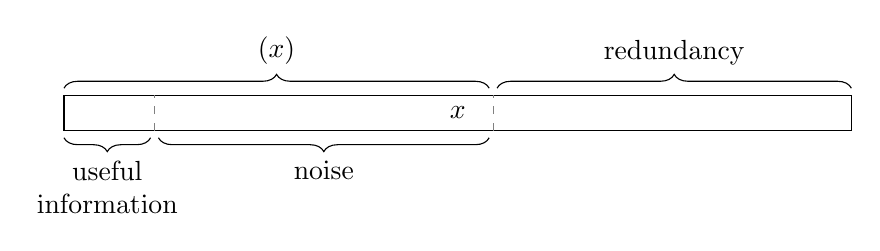
\begin{tikzpicture}[decoration={brace,amplitude=5pt}]
    \draw (0, 0) rectangle (10, 3ex);
    \node at (5, 1.5ex) {$x$};
    \draw[decorate,yshift=2.5pt] (0, 3ex) -- (5.4, 3ex)
      node[midway,above=5pt] {$\KC(x)$};
    \draw[decorate,yshift=2.5pt] (5.5, 3ex) -- (10, 3ex)
      node[midway,above=5pt] {redundancy};
    \draw[decorate,yshift=-2.5pt] (5.4, 0) -- (1.2, 0)
      node[midway,below=5pt] {noise};
    \draw[decorate,yshift=-2.5pt] (1.1, 0) -- (0, 0)
      node[midway,below=5pt,align=center] {useful \\ information};
    \draw[help lines,dashed]
      (1.15, 0) -- ++(0, 3ex)
      (5.45, 0) -- ++(0, 3ex);
  \end{tikzpicture}
  % 11% useful, 43% noise, 46% redundant, like in Example 3.4.2.
  \caption{
    The length of a string~$x$, decomposed into the Kolmogorov complexity of~$x$ and the redundancy in~$x$.
    The Kolmogorov complexity is further decomposed into useful information and useless noise.
    Relative sizes are depicted in accordance with Example~\ref{ex:bmp_png_jpeg}.
  }
  \label{fig:length_decomposed}
\end{figure}

A difference between parameterized algorithmic statistics and the traditional form can be seen in the treatment of random strings.
While the traditional sophistication of a random string is very low, the parameterized sophistication with respect to an informative parameterization~$\eta$ is not.\indexkey{parameterization!informative}
This is a consequence of Theorem~\ref{thm:randomhard} and the fact that the minimization function~$\mu_\eta$ lower bounds the sophistication~$\soph_\eta$.
In other words, what is traditionally considered noise, may become information in the context of a quasiparameterization.
We take this as further evidence supporting Slogan~\ref{slo:useful_information}: useful information is context-dependent.

That random strings may contain a substantial amount of useful information violates one of the original intuitions about what useful information is.
A common perception is that neither strings of minimum Kolmogorov complexity, nor strings of maximum Kolmogorov complexity can be rich in useful information \parencite{adriaans2012facticity}.
Useful information, it is often thought, should strike a balance between these two extremes~\parencite{vitanyi2006meaningful,adriaans2012facticity}.
Challenging this intuition is the goal of lossy data compression, which is to extract of a string its useful information.
When the length of a string is divided into useful information, noise, and redundancy, as in Figure~\ref{fig:length_decomposed}, we observe that useful information is necessarily random.
Therefore, the output of a lossy compression routine is ideally both high in useful information and high in Kolmogorov complexity.
Of course, lossy compression is specific to a certain domain, such as images.
Without knowing this domain, a compressed string may not appear particularly informative.
More generally, contrary to Kolmogorov complexity, a notion of length is wholly determined by the chosen method of encoding.
Since randomness revolves around a comparison between Kolmogorov complexity and length, randomness too is dependent on the chosen method of encoding.
\slogan{There is no such thing as a random object unless the object is a string and nothing but a string.}

Sophistication focuses on sufficient statistics.
Sufficiency of a parameterized models is a robust concept and no hidden additive constants are involved.
Still, we may want to take parameterized models that are nearly sufficient into account in our analysis of the information in a string.
For this, we measure how far away a parameterized model is from being a sufficient parameterized statistic \parencite{vereshchagin2017algorithmic}.
\begin{definition}
  The \defkeyat{parameterized!optimality deficiency}{parameterized optimality deficiency} of a string~$x$ in a parameterized model~$k$ with respect to a quasiparameterization $\eta$ is
  \begin{equation*}
    \updelta_\eta(x, k) \deq \length{\pair{k}{\rank(x : \eta_k)}} - \pc_\eta(x).
  \end{equation*}
  When $k$ is not a parameterized model for~$x$, we set $\updelta_\eta(x, k) \deq \infty$.
\end{definition}
Observe that the parameterized optimality deficiency is~$0$ precisely when the parameterized model is a sufficient parameterized statistic.
On the basis of optimality deficiency, we can express whether a string has parameterized models of a given length that meet a required level of sufficiency.
\begin{definition}
  Let $\alpha$ and $\beta$ be natural numbers and $\eta$ a quasiparameterization.
  A string~$x$ is \defkeyat{parameterized!stochasticity@$(\alpha, \beta)$-stochasticity}{$(\alpha, \beta)$"~$\eta$"~stochastic} if there is an $\eta$"~model~$k$ for~$x$ satisfying
  \begin{equation*}
    \length{k} \le \alpha \quad\text{and}\quad \updelta_\eta(x, k) \le \beta.
  \end{equation*}
\end{definition}
\begin{example}
  \indexkey{example!1729}%
  The number \num{1729} enjoys some fame for being very much not a dull number.
  It is known as the \emph{Hardy--Ramanujan number}, after a visit from Godfrey~H.~Hardey to Srinivasa Ramanujan where the number was discussed.
  At first, it may seem that the number does not have any striking features.
  If we let~$\eta$ be something like a parameterized model class of number theoretic properties.
  We may expect that, when~$k_\text{odd}$ is the $\eta$"~model of odd numbers, the number \num{1729} is $(\length{k_\text{odd}}, \beta)$"~$\eta$"~stochastic for some small value of~$\beta$.
  That is, we may expect that there is not much more to \num{1729} than it being odd.
  However, \num{1729} is the \num{261}st product of three distinct primes.
  While we have not pinned down~$\eta$ exactly, we may expect that being the product of three distinct primes is a fairly simple property.
  As \num{1729} is only the \num{865}th odd number, the parameterized optimality deficiency of \num{1729} in~$k_\text{odd}$ may not be so small after all.
  Instead, we are better off modeling \num{1729} with the $\eta$"~model of products of three distinct primes, $k_{3\text{-primes}}$.
  Still, we may not have that \num{1729} is $(\length{k_{3\text{-primes}}}, \beta)$"~$\eta$"~stochastic for any too small value of~$\beta$.
  This is because \num{1729} is also the first number that is the sum of two cubes of positive numbers in two different ways.
  Thus \num{1729} is the first member of the model of numbers that are the sum of two cubes of positive numbers in multiple ways, $k_{2\text{-cubes}}$.
  While this last model is the most complex, it is quite likely that it determines the sophistication of \num{1729}.
  In summary, we have three $\eta$"~models for \num{1729}, satisfying
  \begin{gather*}
    \length{k_\text{odd}} \le \length{k_{3\text{-primes}}} \le \length{k_{2\text{-cubes}}}, \\
  \shortintertext{and}
    \updelta_\eta(\num{1729}, k_{2\text{-cubes}}) \le \updelta_\eta(\num{1729}, k_{3\text{-primes}}) \le \updelta_\eta(\num{1729}, k_\text{odd}).
  \end{gather*}
\end{example}

Traditionally, stochasticity is not defined using optimality deficiency, but using a slightly different deficiency measure known as \emph{randomness deficiency} \parencite{shen1983concept,li2008introduction}.
These two deficiency measures can differ.
For traditional algorithmic statistics, \textcite[][Theorem~2]{vereshchagin2017algorithmic} have shown that both measures lead to essentially the same notion of stochasticity.
The same holds true for restricted model classes, thanks to a result of \textcite{vereshchagin2010rate} \parencite[see also][]{vereshchagin2017algorithmic}.
Because it fits our framework better, we therefore prefer optimality deficiency over randomness deficiency.

Let us take a look at the stochasticity of a string $x$ in relation to a quasiparameterization $\eta$.
The values of $\alpha$ and $\beta$ for which $x$ is $(\alpha, \beta)$"~$\eta$"~stochastic partition the plane \parencite{vereshchagin2004kolmogorov,gacs2001algorithmic}.
Suppose that $\alpha$ and $\beta$ are so that $x$ is $(\alpha, \beta)$"~$\eta$"~stochastic.
There is then an $\eta$"~model of complexity at most $\alpha$ that is within $\beta$ of being a sufficient parameterized statistic for $x$.
Sometimes, relaxing the sufficiency requirement slightly means that simple models become available.
Thus, a string $x$ may be $(\alpha, \beta)$"~$\eta$"~stochastic for values of $\alpha$ and $\beta$ that are reasonably small in relation to its length $\length{x}$.
Such a string $x$ is informally said to be \emph{stochastic} \parencite{vereshchagin2017algorithmic}.

\begin{example}
  \indexkey{example!image compression}%
  In Example~\ref{ex:useful_information}, we encountered the JPEG lossy image compression format.
  The JPEG compression procedure contains a tuning parameter that determines the amount of degradation in quality that is considered admissible.
  This tuning parameter can range in value from $1$ to $100$, where $100$ represents near-perfect reproduction of the original image.
  Unfortunately, there is no unique minimal value of this parameter for which the degradation in image quality is unnoticeable.
  In other words, there is no clear-cut quality value beyond which a JPEG compressed image is a sufficient statistic for the original image.
  For Example~\ref{ex:useful_information}, a quality value of $90$ was used.

  With a lower quality setting, the JPEG compression procedure is able to produce smaller files.
  The compressed file size can be thought of as the size of a model for the original image.
  Thus, the $\alpha$ component of stochasticity acts like a bound on on the file size.
  Because there is no proper sufficiency criterion for JPEG compression, the quality setting cannot directly be related to the $\beta$ component of stochasticity.
  However, there is a conceptual connection between lowering the quality setting and increasing the value of $\beta$.

  \begin{figure}
    \centering
    \begin{tikzpicture}
      \begin{axis}[
        width=10cm,
        no markers,
        xlabel={JPEG quality setting},
        ylabel={mean compressed file size (kilobytes)},
      ]
        \addplot table [y expr={\thisrowno{1}/1000}] {kodak.dat};
      \end{axis}
    \end{tikzpicture}
    \caption{
      The mean file size of the images in the Kodak True Color Image Suite~\parencite{franzen1999kodak} after JPEG compression at different quality settings.
    }
    \label{fig:jpeg_q}
  \end{figure}
  We are used to seeing a substantial decrease in file size when we allow the image quality to degrade only slightly.
  In Figure~\ref{fig:jpeg_q}, this can indeed be observed.
  At high values of the quality parameter, small changes have a large impact on the resulting file size.
\end{example}

The traditional notion of stochasticity is a special case of our parameterized one.
A string is called $(\alpha, \beta)$"~stochastic, without mention of any $\eta$, if it is stochastic in relation to the parameterization given~by~\eqref{eq:quasi_decision}.
Not all strings are stochastic.
In fact, some of the strings of which the sophistication is close to the length are not stochastic at all.
Extending a similar result by \textcite{shen1983concept}, it was shown that some strings are only $(\alpha, \beta)$"~stochastic when $\alpha + \beta$ nearly exhausts the length of the string \parencite{gacs2001algorithmic}.
More specifically, for each $n$, there is a string of length $n$ that is only $(\alpha, \beta)$"~stochastic when $\alpha + \beta$ is at least $n - \bigO(\log n)$.
This result about the existence of non-stochastic strings can be extended to the parameterized form of stochasticity.
\begin{theorem}
\label{thm:stochastic}%
  Let $x$ be a string, $\eta$ a decidable quasiparameterization, and $\KC(\eta)$ the minimum length of a decision procedure for $\eta$.
  Furthermore, define $\gamma \deq \pc_\eta(x) - \KC(x)$, which is so that $\eta$ captures the complexity of $x$ if $\gamma$ equals $0$.
  If $x$ is $(\alpha, \beta)$"~$\eta$"~stochastic, then it is $(\alpha + \KC(\eta), \beta + \gamma + \KC(\eta))$"~stochastic.
\end{theorem}
\begin{proof}
  Let $k$ be an $\eta$"~model for $x$ witnessing that $x$ is $(\alpha, \beta)$"~$\eta$"~stochastic and let $j$ be the encoding of a decision procedure for $\eta_k$ of minimum length.
  Recall from Example~\ref{ex:traditional_pc} that parameterized complexity in the traditional setting equals Kolmogorov complexity and observe that we have
  \begin{equation*}
    \length{j} \le \length{k} + \KC(\eta) \le \alpha + \KC(\eta).
  \end{equation*}
  It remains to show that the optimality deficiency of $x$ in $k$ with respect to $\eta$ is at most $\beta + \gamma + \KC(\eta)$.
  The first step to this end follows the same reasoning as we have just encountered,
  \begin{align*}
    \updelta(x, j) &= \length{\pair{j}{\rank(x : \eta_k)}} - \KC(x) \\
    	&\le \length{\pair{k}{\rank(x : \eta_k)}} + \KC(\eta) - \KC(x)
  \intertext{which can then be expanded as}
    	&= \length{\pair{k}{\rank(x : \eta_k)}} + \KC(\eta) - \pc_\eta(x) + \gamma \\
    	&= \updelta_\eta(x, k) + \gamma + \KC(\eta) \\
    	&\le \beta + \gamma + \KC(\eta).
  \end{align*}
  Thus, $\eta_k$ witnesses that $x$ is $(\alpha + \KC(\eta), \beta + \gamma + \KC(\eta))$"~stochastic.
\end{proof}
When~$\eta$ is held fixed, $\KC(\eta)$ is constant and disappears in the theorem above.
The constant~$\gamma$ depends on~$x$ and only disappears when~$\eta$ captures the complexity of~$x$.
If the complexity of a non-stochastic string~$x$ is captured by a quasiparameterization~$\eta$, then $x$ is also non-$\eta$"~stochastic.
This follows from the contrapositive formulation of Theorem~\ref{thm:stochastic}.
\begin{corollary}
\label{cor:nonstochastic}%
  Let $x$ be a string and $\eta$ a decidable quasiparameterization.
  Furthermore, let $\gamma = \pc_\eta(x) - \KC(x)$ be the amount by which the complexity of~$x$ escapes~$\eta$.
  If $x$ is not $(\alpha, \beta)$"~stochastic, then it is not $(\alpha - \KC(\eta), \beta - \gamma - \KC(\eta))$"~$\eta$"~stochastic either.
\end{corollary}

The quasiparameterization defined in~\eqref{eq:quasi_decision} includes $\binary^+$ as a model.
Therefore, the minimization function with respect to that quasiparameterization is bounded by a constant.
The same is not true of the sophistication.
Put differently, there is a constant~$\alpha$ such that for every string~$x$ there is a constant~$\beta_x$ such that $x$ is $(\alpha, \beta_x)$"~stochastic.
This constant,~$\beta_x$, cannot be bounded from above independent of~$x$.
The same cannot be said for stochasticity with respect to an arbitrary quasiparameterization~$\eta$.
A string may fail to be $\eta$"~stochastic not only because simple $\eta$"~models are not good enough, but also because the string has no simple $\eta$"~models.
For all $\alpha < \mu_\eta(x)$, regardless of~$\beta$, the string~$x$ is not $(\alpha, \beta)$"~$\eta$"~stochastic.
The sophistication of~$x$ with respect to~$\eta$ may even be bigger than its length, $\soph_\eta(x) > \length{x}$.
For such~$x$ and~$\eta$, there are values of~$\beta$ with which~$x$ is not even $(\length{x}, \beta)$"~$\eta$"~stochastic.
Consequently, $\eta$ does not capture the complexity of~$x$ and the non"~$\eta$"~stochasticity of~$x$ is not a consequence of Corollary~\ref{cor:nonstochastic}.
Indeed, there would be no reason to assume that $x$ is non-stochastic in the traditional sense.

\subsection{Parameter Estimation}
\label{sec:estimation}%
In Lemma~\ref{lem:pccomputable}, we found that the parameterized complexity with respect to a decidable quasiparameterization is computable.
Not only does this result extend to the computability of sophistication, it also entails that optimality deficiency is computable.
Therefore, for a fixed~$\alpha$ and~$\beta$, and a decidable~$\eta$, the set of $(\alpha, \beta)$"~$\eta$"~stochastic strings is decidable.
Moreover, for an $(\alpha, \beta)$"~$\eta$"~stochastic string~$x$, a witness of its stochasticity can be computed.
In particular, for the case where $\beta$ equals $0$, we can compute an $\eta$"~model~$k$ for~$x$ such that we have $\length{k} = \soph_\eta(x)$.
In terms of statistics, a mapping from~$x$ to an $\eta$"~model for~$x$ is an \defkey{estimator}.
Indeed, the model class conveyed by~$\eta$ is parametric also in the statistical sense.
This probabilistic interpretation of concepts in algorithmic statistics has been recognized early on \parencite{rissanen1983universal,vitanyi2000minimum,gacs2001algorithmic}.
An estimator that realizes the sophistication of its input is particularly exciting, as its output is a sufficient statistic that is as simple as can be.
While computable with respect to decidable quasiparameterizations, the computation of such an estimator may be prohibitively resource intensive.
For this reason, alternative estimators and their advantages and disadvantages are studied.

So far, underlying our investigation has been a two-part code for describing a string~$x$.
If~$k$ is an $\eta$"~model for~$x$, then, knowing~$\eta$, we can recover~$x$ from
\begin{equation}
\label{eq:two-part}
  \pair{k}{\rank(x : \eta_k)}.
\end{equation}
We can minimize several quantities related to this two-part specification and each defines a different estimator.
The simplest model for~$x$ is one that minimizes the length of the first part of the specification, $\length{k}$.\indexkey{Occam's razor}
The corresponding~$k$ can be called the \defkeyat{estimator!Occam's razor}{Occam's razor} estimate, and its length equals~$\mu_\eta(x)$.
In traditional algorithmic statistics, this estimator is of no interest because the complexity of the simplest model for a string cannot exceed that of~$\binary^+$.
However, in parameterized algorithmic statistics, $\binary^+$ need not occur as a slice in any specific quasiparameterization.
Rather than minimizing the length of the first part of the specification, we could also minimize the length of the second part, $\length{\rank(x : \eta_k)}$.
The corresponding $\eta$"~model~$k$ is one that contains as much information about~$x$ as possible, and is known as the \defkeyat{estimator!maximum likelihood}{maximum likelihood} estimate \parencite{vereshchagin2004kolmogorov}.
In traditional algorithmic statistics, this estimator would yield a model of which the input string is the first element.
Again, in parameterized algorithmic statistics, such a model need not occur as a slice in any given quasiparameterization.
Minimizing the total length of the two-part specification of~$x$, we recover the \defkeyat{estimator!minimum description length}{minimum description length} estimator.\indexkey{minimum description length}
Equivalently, this estimator minimizes the sum of the lengths of both parts and as such balances the previous two estimators \parencite{vereshchagin2004kolmogorov,rissanen1983universal}.
An estimate obtained by this estimator is a sufficient statistic.
When we restrict to the simplest such models, we find that the length of a minimum description length estimate~$k$ is the sophistication $\soph_\eta(x)$.
In summary, some natural estimators derived from the two-part description of a string, and their minimization objectives, are the following.
\begin{center}
  \begin{tabular}{r@{ }lcc}
    \multicolumn{2}{c}{\emph{estimator}}	& \emph{minimizes}	& \emph{length} \\
    \hline
    Occam's razor&(OR)	& first part	& $\mu_\eta$ \\
    maximum likelihood&(ML)	& second part	& \footnotesize{[no name]} \\
    minimum description length&(MDL)	& sum	& $\soph_\eta$
  \end{tabular}
\end{center}

The parameterization defined by~\eqref{eq:quasi_decision} is not decidable and traditional algorithmic statistics pays attention to the computability of estimators.
One approach to the computability of estimators is to place an upper bound on the model complexity and consider each estimator as a function of this bound \parencite{gacs2001algorithmic,vereshchagin2004kolmogorov} \parencite[in the presence of resource bounds,][]{milovanov2017algorithmic}.
Specifically, we consider ML and MDL relative to a quasiparameterization consisting of a selection of the slices of~\eqref{eq:quasi_decision}.
The selection is obtained by including only those models of which the corresponding parameter value has a length shorter than the anticipated bound.
As mentioned before, OR is not interesting in the traditional context because it can be upper bounded by a constant.
On the other hand, ML and MDL are interesting, but, while the length of their estimates can be approximated from above, they are not computable~\parencite{vereshchagin2004kolmogorov}.
Of the two estimators, MDL is easier to approximate and therefore more convenient to work with in practice \parencite[][Section~V.B]{vereshchagin2004kolmogorov}.
Additionally, as a function of a bound on the model complexity, MDL selects a sufficient statistic precisely when ML does \parencite[][Lemma~IV.2]{vereshchagin2004kolmogorov}.
With respect to decidable parameterizations, OR, ML, and MDL would all be computable as a function of a bound on the length of parameter values.
Note, though, that without such a bound ML need not be computable.
Unfortunately, in the parameterized setting MDL cannot simply be used as a substitute for ML.
The tight correspondence between the two in traditional algorithmic statistics is not a given in the parameterized setting.

There are many more estimators than the three we have looked at so far, OR, ML, and MDL.
For a quasiparameterization~$\eta$, we may look at those estimators that are in some sense consistent with~$\eta$.
\begin{definition}
  A function $\kappa\colon \binary^+ \to \binary^+$ is a \defkeyat{estimator!parameter estimator}{parameter estimator} for a quasiparameterization~$\eta$ if it is consistent with $\eta$ in the sense that, for all strings~$x$, we have $x \in \eta_{\kappa(x)}$
\end{definition}
\begin{example}
  Suppose $\kappa$ is a parameterization in the \citeauthor{flum2006parameterized} framework for parameterized complexity theory.
  On page~\pageref{eq:flum_parameterization}, we associated with this function the parameterization
  \begin{equation*}
    \eta \deq (\{x \st \asNat(\kappa(x)) \le \asNat(k)\})_{k \in \binary^+}.
  \end{equation*}
  For this parameterization, $\kappa$ is a polytime-computable parameter estimator.
\end{example}

We have seen that when~$\eta$ is decidable, the parameter estimators OR and MDL are computable.
Yet, even when $\eta$ is not decidable, a parameter estimator for~$\eta$ may be computable.
For instance, if $\kappa$ maps all strings to an encoding of a decision procedure for $\binary^+$, it is a computable parameter estimator for~\eqref{eq:quasi_decision}.

\begin{example}[continued from Example~\ref{ex:p-cylinder}]
  \indexkey{example!p-cylinder@\pdash{}cylinder}%
  Let $A$ be a \pdash{}cylinder and $g\colon \binary^+ \to \binary^+ \times \binary^+$ a corresponding isomorphism.
  Recall that the parameterization based on $g$ was defined as
  \begin{equation*}
    \eta \deq (\{x \st \asNat(g_1(x)) \le \asNat(k)\})_{k \in \binary^+}.
  \end{equation*}
  For this parameterization, $g_1$ is a parameter estimator.
  As $g_1$ is computable in polynomial time, it is also a parameterization in the sense of \citeauthor{flum2006parameterized}.
  Moreover, we have, for all $x$,
  \begin{equation*}
    \mu_\eta(x) = \soph_\eta(x) = \length{g_1(x)}.
  \end{equation*}
  Note that~\eqref{eq:compatible_strong} holds for~$\eta$, so we find that OR, ML, MDL, and $g_1$ are all the same parameter estimator for~$\eta$.
\end{example}

Using computable parameter estimators we can obtain a lower bound on the Kolmogorov complexity of a string.
Since~\eqref{eq:soph} extends to parameterized complexity,
\begin{equation}
\label{eq:kclepc}
  \KC(x) \le \pc_\eta(x) + \KC(\eta),
\end{equation}
a bound on the Kolmogorov complexity can be turned into a bound on the parameterized complexity.
This, then, will allow us to upper bound the parameterized optimality deficiency using a computable parameter estimator~$\kappa$.

Bounding the Kolmogorov complexity of a string using a computable parameter estimator~$\kappa$ is possible via the inverse images of~$\kappa$.
Since $\kappa$ is computable, for every parameter value~$k$, the inverse $\kappa^{-1}(k) = \{x \st \kappa(x) = k\}$ is a decidable set.
Therefore, letting $\KC(\kappa)$ denote the minimum length of a procedure for computing~$\kappa$, we have, for every string~$x$ and with $k = \kappa(x)$,
\begin{equation}
\label{eq:kclowerbound}
  \KC(\pair{k}{\rank(x : \kappa^{-1}(k))}) \le \KC(x) + \KC(\kappa).
\end{equation}
Specifically, from $x$ we can compute $k$ and $\rank(x : \kappa^{-1}(k))$, so the complexity of those values together is at most that of~$x$ plus that of~$\kappa$.
It should be noted that $\kappa^{-1}(k)$ need not be a slice of the quasiparameterization~$\eta$.
However, this is mainly a technical concern as we can extend $\eta$ to include these inverses for all parameter values.
Given~$\eta$ and a parameter estimator~$\kappa$ for $\eta$, let~$\eta'$ be the quasiparameterization defined by
\begin{equation*}
  \eta'_{k'} \deq \begin{cases}
    \eta_k	&\text{if $k' = \bits{0}k$}, \\
    \kappa^{-1}(k)	&\text{if $k' = \bits{1}k$}.
  \end{cases}
\end{equation*}
If $\eta$ is decidable and $\kappa$ is computable, then $\eta'$ is decidable too.
Moreover, it is in the same equivalence class as $\eta$ in the uniform order on parameterizations defined in Definition~\ref{def:uniform_order}.
For completeness, we lift the parameter estimator~$\kappa$ to a parameter estimator~$\kappa'$ defined by $\kappa'(x) \deq \bits{1}\kappa(x)$.
This turns a computable parameter estimator~$\kappa$ for~$\eta$ into a computable parameter estimator~$\kappa'$ for~$\eta'$ in a way that we have, for any string $x$,
\begin{equation*}
  \eta'_{\kappa'(x)} = \kappa'^{-1}(\kappa'(x)).
\end{equation*}

Let us say that a parameter estimator~$\kappa$ for a quasiparameterization~$\eta$ that, for all~$x$, satisfies $\eta_{\kappa(x)} = \kappa^{-1}(\kappa(x))$ is a \defkeyat{estimator!slice-estimator}{slice"~estimator}.
We then get the following theorem that allows us to identify $\eta$"~stochastic strings.
\begin{theorem}
\label{thm:etastochastic}%
  Let $\eta$ be a decidable quasiparameterization, $\kappa$ a computable slice"~estimator for~$\eta$.
  There is a constant $c$ such that, for any string~$x$, when we set
  \begin{align*}
    k &\deq \kappa(x), \\
    i &\deq \rank(x : \kappa^{-1}(k)), \\
    \beta &\deq \length{\pair{k}{i}} - \KC(\pair{k}{i}) + c,
  \end{align*}
  we find that $x$ is $(\length{k}, \beta)$-$\eta$-stochastic.
\end{theorem}
\begin{proof}
  The claimed parameterized stochasticity is witnessed by the slice $\eta_k = \kappa^{-1}(k)$.
  To see that the parameterized optimality deficiency of~$x$ with respect to~$\eta$ is indeed at most~$\beta$, consider
  \begin{align*}
    \updelta_\eta(x, k) &= \length{\pair{k}{\rank(x : \eta_k)}} - \pc_\eta(x) \\
      &= \length{\pair{k}{i}} - \pc_\eta(x) \\
    \intertext{which, by~\eqref{eq:kclepc} and~\eqref{eq:kclowerbound}, satisfies}
      &\le \length{\pair{k}{i}} - (\KC(x) - \KC(\eta)) \\
      &\le \length{\pair{k}{i}} - \KC(\pair{k}{i}) + \KC(\eta) + \KC(\kappa).
  \end{align*}
  As $\KC(\eta)$ and $\KC(\kappa)$ are independent of $x$, we may set $c \deq \KC(\eta) + \KC(\kappa)$, with which the last line becomes to equal $\beta$ and the bound is proven.
\end{proof}

Of course, a string should only be called $\eta$"~stochastic if it has a simple model with a low optimality deficiency.
To see that Theorem~\ref{thm:etastochastic} can truly be used to identify $\eta$"~stochastic strings, we first take a closer look at the optimality deficiency.
Observe that $\length{\pair{k}{i}}$ can be arbitrarily large, while $\KC(\pair{k}{i})$ is still small.
In fact, for any constant~$c$ and any sufficiently large~$\beta$, there are infinitely many values of~$k$ and~$i$ such that we have
\begin{equation*}
  \length{\pair{k}{i}} - \KC(\pair{k}{i}) + c \le \beta.
\end{equation*}
In fact, the incompressibility theorem for algorithmic prefix complexity \parencite[][Theorem~3.3.1(ii)]{li2008introduction} tells us that the inequality must hold for a large fraction of possible values of~$k$ and~$i$.
Specifically, for each fixed constant~$r$, of all $\pair{k}{i}$ of length $n$, at most $2^{n - r + \bigO(1)}$ satisfy $r \le \length{\pair{k}{i}} - \KC(\pair{k}{i})$.
Moreover, this is still true of all the possible values of~$i$ after we fix a value of~$k$ \parencite[][Theorem~3.9.1]{li2008introduction}.
Thus, we can turn Theorem~\ref{thm:etastochastic} into a statement about the prevalence of stochastic strings.
\begin{corollary}
\label{cor:stochastic}%
  Let $k$ be an infinite $\eta$"~model in the range of~$\kappa$.
  For all~$\beta$, among the first $m$ elements of~$\eta_k$ at least $(1 - 2^{-c})m$ are $(\length{k}, \beta)$"~$\eta$"~stochastic, where~$c$ equals $\beta - \bigO(1)$ with the final term depending on $\eta$, $\kappa$, and $k$.
\end{corollary}
Note that, for a fixed value of~$\beta$, the dependence on~$k$ of the hidden constant is more specifically a dependence on~$\length{k} - \KC(k)$.
Because of that, the corollary is especially powerful when the range of~$\kappa$ contains an infinite random set of parameter values belonging to infinite $\eta$"~models.
In that case, the same density of strings with an optimality deficiency bounded by~$\beta$ is achieved on infinitely many $\eta$"~models.
Informally, disregarding the density considerations, the corollary can then be phrased in a way that somewhat resembles the instance complexity conjecture:\indexkey{instance complexity conjecture}
Infinitely many $\eta$"~models are a near-sufficient parameterized statistic infinitely often.
More concretely, this means that the situation where a parameter value contains all useful information about a string and nothing more occurs infinitely often.
\slogan{Infinitely many parameter values reflect precisely all useful information of infinitely many strings.}

Moreover, if $\pair{k}{i}$ is a random string in the sense that we have $\length{\pair{k}{i}} = \KC(\pair{k}{i})$, then \eqref{eq:kclowerbound} becomes an equality.
In that case, the quasiparameterization~$\eta$ captures the complexity of the $\eta$"~stochastic strings considered in Corollary~\ref{cor:stochastic}.
We point out that if $\eta$ is informative, then this set of strings of which $\eta$ captures the complexity is not a random set.
Likewise, if the slices of $\eta$ are sparse, then most of these strings of which $\eta$ captures the complexity are highly non-random.

\begin{example}[continued]
\label{ex:simultaneous}%
  \indexkey{example!p-cylinder@\pdash{}cylinder}%
  By capturing the complexity of a string, a quasiparameterization isolates the redundancy in the description of a string into the second part of a two-part code.
  Originally, however, parameterized complexity theory did not target algorithmic complexity.
  Instead, it revolved around isolating not descriptive redundancy, but computational redundancy associated with a string in light of a decision problem.
  It is worthwhile to note that a quasiparameterization can achieve both these feats simultaneously.

  Let $A$ be a \pdash{}cylinder, $g\colon \binary^+ \to \binary^+ \times \binary^+$ a corresponding isomorphism and $\eta$ the quasiparameterization based on $g$.
  All slices of $\eta$ are infinite and the range of $g_1$ is the entire set $\binary^+$.
  Because of this, it follows from Corollary~\ref{cor:stochastic} that infinitely many slices of $\eta$ contain infinitely many strings of which $\eta$ captures the complexity.
  For those strings, $\eta$ acts as a measure of both algorithmic and computational complexity.
\end{example}

A parameterization can witness that computational and algorithmic complexity may coincide infinitely often.
However, this does not provide us with a dual to Theorem~\ref{thm:randomhard}.
While some strings of low algorithmic complexity may appear in a parameterization with short parameter values, this need not be true of all such strings.
In order to control the expected minimum length of a parameter value for a given string, we need to tinker with the distribution we use to sample the strings.

\subsection{Encodings and Distributions}
\label{sec:encodings_distributions}%
At the end of Section~\ref{sec:stochasticity}, several possibilities were discussed for why a string may fail to be stochastic with respect to a quasiparameterization~$\eta$.
While any of these may be used to prove that non-$\eta$"~stochastic strings exist, they tell us very little about how likely we are to encounter such strings.
The existence of non-stochastic strings in the traditional sense is described by \citeauthor{vereshchagin2017algorithmic} as a \enquote{mathematical existence result; it does not say anything about the possibility to observe non-stochastic objects in the \enquote{real world}}.
In support of this sentiment, they show that any effective way of sampling from~$\binary^+$ may produce a non-stochastic string only with a negligible probability \parencite{muchnik1998mathematical,vereshchagin2017algorithmic}.
This result makes use of the universal probability distribution, which is the distribution related to Kolmogorov complexity via the Kraft inequality.\indexkey{Kraft~inequality}
A similar result revolving around the cardinality of the set of non-stochastic strings goes back to \textcite[][Theorem~3]{shen1983concept}.
For parameterized algorithmic statistics, a bound on the cardinality of the set of non-$\eta$"~stochastic strings is available in the form of Corollary~\ref{cor:stochastic}.
However, we should not expect any results building on the universal distribution.
In our framework, we use the slices of quasiparameterizations as a substitute for the decidable sets.
Hence, our reference measure of algorithmic complexity should be parameterized complexity instead of Kolmogorov complexity.
We shall explore distributions derived from parameterized complexity, and their effect on the parameter values we may expected for strings of a given length.

\subsubsection{The Uniform Distribution}
For a start, if we assume all strings of length~$n$ are equally likely, the effects of Corollary~\ref{cor:stochastic} are canceled by Theorem~\ref{thm:randomhard}.
The random strings alone push the expected minimum length of a parameter value to within a multiplicative constant of its maximum value.
\begin{theorem}
\label{thm:expected_uniform}%
  Let $\eta$ be an informative parameterization and consider the expected value of $\mu_\eta(x)$, conditional to the length of $x$, under the uniform distribution on strings of a given length, $\Ex_\mathrm{unif}(\mu_\eta(x) \given \length{x})$.
  There is a constant~$c$ such that, for all~$n$, we have
  \begin{equation*}
    \Ex_\mathrm{unif}(\mu_\eta(x) \given \length{x} = n) \ge \frac{\upM_\eta(n)}{c} - c.
  \end{equation*}
\end{theorem}
\begin{proof}
  Pick a constant~$r$, fix an arbitrary value for~$n$, and let $X$ be the random set $\{x \in \binary^n \st \KC(x) \ge n + \KC(n) - r\}$.
  By Theorem~\ref{thm:randomhard}, there is a constant~$h$, independent of~$n$, such that all $x \in X$ satisfy $\mu_\eta(x) \ge \upM_\eta(n) - h$.
  Further, the incompressibility theorem~\parencite{li2008introduction} tells us that $X$ contains at least $2^n(1 - 2^{-r + \bigO(1)})$ strings.
  Together, these observations make the following derivation possible.
  \begin{align*}
    \Ex_\mathrm{unif}(\mu_\eta(x) \given \length{x} = n) &= \sum_{x \in \binary^n} \mu_\eta(x) \cdot 2^{-n} \\
      &\ge \sum_{x \in X} \mu_\eta(x) \cdot 2^{-n} \\
      &\ge \sum_{x \in X} (\upM_\eta(n) - h) \cdot 2^{-n} \\
      &\ge 2^n \cdot (1 - 2^{-r + \bigO(1)}) \cdot (\upM_\eta(n) - h) \cdot 2^{-n} \\
      &\ge (1 - 2^{-r + \bigO(1)}) \cdot \upM_\eta(n) - h.
  \end{align*}
  Now, choosing $c = \max\left\{\frac{1}{1 - 2^{-r + \bigO(1)}}, h\right\}$, we get the statement of the theorem.
\end{proof}

For parameterizations encountered in practice, we often have $\upM_\eta(n) \in \bigO(\log n)$.
This is because the parameter value~$k$ of minimal length with which a string~$x$ is in $\eta_k$ is usually so that $\asNat(k)$ can be bounded by a polynomial in $\length{x}$.
The vertex cover parameterization considered in Example~\ref{ex:vc_informative} is an example of such a parameterization.
Moreover, this bound on~$\upM_\eta$ is usually tight, meaning that there are constants~$c_1$ and~$c_2$ such that, for all~$n$, we have $c_1 \log n \le \upM_\eta(n) \le c_2 \log n$.
Now, Theorem~\ref{thm:expected_uniform} says that the same is true of the expected value of $\mu_\eta(x)$.
This translates to the fact that $\length{x}$ can be bounded from above by a polynomial in the expected value of $\asNat(k)$.
Now, suppose $\phi$ is a parameterized procedure with a fixed-parameter tractable running time of $f(k)\length{x}^{\bigO(1)}$, for some function~$f$.
By Jensen's inequality~\parencite{cover2006elements}, we find $\Ex(f(k) \given \length{x}) \ge f(\Ex(k \given \length{x}))$, insofar the expected value of a string would make any sense.
Consequently, the expected running time of~$\phi$, assuming a uniform distribution on the strings of a given length, is comparable to the worst-case running time.
As this is not what we observe in practice, we should take parameter values into account in the distributions we consider.

\subsubsection{The Random--Hard Distribution}
Increasing the role of the parameter value, we can use the encoding that we came across in the proof of Theorem~\ref{thm:randomhard} as the basis of a distribution.
The multi-part encoding described there may allow for several different encodings of a single string~$x$.
This is because there may be multiple parameter values~$k$, each of length at most $\upM_\eta(\length{x})$, such that $x$ is included in~$\eta_k$.
We shall take all possible encodings into account in our distribution.
Specifically, we define our distribution so that the probability of a string~$x$ is the that of generating a description of~$x$ by means of tossing a fair coin.
For any string~$x$, let $S_x$ be the set of possible parameter values with which $x$ can be encoded, namely
\begin{equation*}
  S_x \deq\{k \st \length{k} \le \upM_\eta(x) \reland x \in \eta_k\}.
\end{equation*}
Using this set, the probability of a string~$x$ in accordance with the encoding used in the proof of Theorem~\ref{thm:randomhard}, the \emph{random--hard} probability, can be expressed as
\begin{align*}
  \Pr_\mathrm{r"~h}(x) &\deq \sum_{k \in S_x} 2^{-(\KC(\length{x}) + \upM_\eta(\length{x}) + 1 + \log \upN_\eta(\length{x}, k))} \\
    &= \frac{1}{2^{\KC(\length{x}) + \upM_\eta(\length{x}) + 1}} \sum_{k \in S_x} \frac{1}{\upN_\eta(\length{x}, k)}
\end{align*}
Note that we have omitted the length of a specification of the parameterization~$\eta$.
As each encoding of every string starts with the same specification of~$\eta$, the encoding still satisfies the Kraft inequality without a specification of~$\eta$.
We obtain the probability conditional to the length of the string by simply dropping the specification of the length, $\KC(\length{x})$.
Thus, for all $n$ and all~$x$ of length~$n$, we have
\begin{equation*}
  \Pr_\mathrm{r"~h}(x \given \length{x} = n) = \frac{1}{2^{\upM_\eta(n) + 1}} \sum_{k \in S_x} \frac{1}{\upN_\eta(n, k)}
\end{equation*}

Typically, slices corresponding to parameter values with a short length contain fewer strings than those corresponding to parameter values with a longer length.
Therefore, the above probability distribution assigns higher probability to strings that occur in a slice for which the parameter value has a short length.
The random--hard probability distribution is the marginal distribution of the strings~$x$ as part of pairs of strings and parameter values, $\pair{k}{x}$.
Here, the parameter values are restricted in length to at most $\upM_\eta(\length{x})$.
Because the distribution is a marginal distribution, it is not straightforward to work with the expected minimum length of a parameter value, $\mu_\eta(x)$.
Therefore, we shall initially consider the expected length of a parameter value, $\length{k}$.
Unfortunately, the expected parameter value length is essentially its maximum value.
\begin{theorem}
\label{thm:expected_randomhard}%
  Let $\eta$ be a quasiparameterization and consider the expected length of a parameter value $k \in S_x$, conditional to the length of $x$, under the random--hard probability distribution.
  For all~$n$, we have
  \begin{equation*}
    \Ex_\mathrm{r"~h}(\length{k} \given \length{x} = n) \ge \upM_\eta(n) - 1.
  \end{equation*}
\end{theorem}
\begin{proof}
  By changing the summation order in the computation of the expected value, we get rid of anything specific to the string~$x$,
  \begin{align*}
    \Ex_\mathrm{r"~h}(\length{k} \given \length{x} = n)
      &= \sum_{x \in \binary^n} \sum_{k \in S_x} \length{k} \frac{1}{2^{\upM_\eta(n) + 1} \upN_\eta(n, k)} \\
      &= \sum_{k\text{ with }\length{k} \le \upM_\eta(n)}\;\sum_{x \in \binary^n \cap \eta_k} \length{k} \frac{1}{2^{\upM_\eta(n) + 1} \upN_\eta(n, k)} \\
      &= \sum_{k,\ \length{k} \le \upM_\eta(n)} \length{k} \frac{1}{2^{\upM_\eta(n) + 1} \upN_\eta(n, k)} \sum_{x \in \binary^n \cap \eta_k} 1 \\
      &= \sum_{k,\ \length{k} \le \upM_\eta(n)} \length{k} \frac{1}{2^{\upM_\eta(n) + 1} \upN_\eta(n, k)} \upN_\eta(n) \\
      &= \frac{1}{2^{\upM_\eta(n) + 1}} \sum_{k,\ \length{k} \le \upM_\eta(n)} \length{k}.
  \end{align*}
  In the last expression, we recognize the expected length of a string of length at most~$\upM_\eta(n)$, where all candidate strings are equally likely.
  To be exact, the full expression equals $\upM_\eta(n) - 1 + \frac{1}{2^{\upM_\eta(n)}}$.
\end{proof}

It is possible to only consider encodings of a string~$x$ with respect to a specific witness of~$\mu_\eta(x)$.
The previous theorem would then become a statement about the expected value of $\mu_\eta(x)$.
For this, consider the boundary of a quasiparameterization $\eta$ defined by\indexkey{parameterization!boundary ($\eta^\partial$)}
\begin{equation*}
  \eta^\partial_k \deq \eta_k \setminus \bigcup_{j < \asNat(k)} \eta_{\asStr(j)}.
\end{equation*}
A string is included in a slice $k$ of this boundary of~$\eta$ only if $\eta_k$ is the first slice of $\eta$ to include $x$.
Thus, the only parameter value with which a string is in the boundary of a quasiparameterization is a shortest parameter value.
The boundary of a quasiparameterization is not itself a quasiparameterization.
However, if a quasiparameterization $\eta$ is decidable, than so is its boundary $\eta^\partial$.
We can use the boundary of a quasiparameterization to define a distribution along the lines of the random--hard distribution discussed previously.
With respect to this distribution, the expected value of $\mu_\eta(x)$ is at least $\upM_\eta(n) - 1$, by Theorem~\ref{thm:expected_randomhard}.
Note that only the distribution has changed and not the reference quasiparameterization~$\eta$ in~$\mu_\eta$ and~$\upM_\eta$.

\subsubsection{Parameterized Complexity Distributions}
With the distributions considered so far, non-$\eta$"~stochastic strings are more prevalent than what we observe in practice.
Let us turn to the two-part code~\eqref{eq:two-part} underlying parameterized complexity.
By varying the pairing function, we get various probability distribution on strings via the Kraft~inequality.
Guided by fixed-parameter tractability, we shall characterize suitable pairing functions.

Assume that the number of bits a pairing function uses to encode each of the components of a pair is independent of the value of the other component.
That is, for all $k$ and $i$, the number of bits required for encoding~$k$ in $\pair{k}{i}$ can be expressed as a function of~$k$ alone, and vice-versa for~$i$.
Let $\ell_1$ and $\ell_2$ be these functions.
Further, let~$A$ be a set that is in~\cl{FPT} with a parameterization~$\eta$ and let $f$ witness the parameter-dependence of the corresponding running time.
We are interested in the expected value of this running time as we know from experience that the expected running times are tractable.
The general form of this expected value with respect to the parameterized complexity distribution, before specifying a pairing function, is
\begin{align*}
  \Ex_\mathrm{pc}(f(k) \given \length{x} = n)
    &= \sum_{k \in \binary^+}\;\sum_{x \in \binary^n \cap \eta_k} f(k) \cdot 2^{-\length{\pair{k}{\rank(x : \eta_k)}}} \\
    &= \sum_{k \in \binary^+} f(k) \cdot 2^{-\ell_1(k)} \sum_{x \in \binary^n \cap \eta_k} 2^{-\ell_2(\rank(x : \eta_k))}.
  \intertext{The final sum is a sum of probabilities, which is at most~$1$, thus we find}
  \Ex_\mathrm{pc}(f(k) \given \length{x} = n)
    &\le \sum_{k \in \binary^+} f(k) \cdot 2^{-\ell_1(k)}.
\end{align*}
Observe that the bounding value on the right is not sensitive to the length~$n$.
Still, it is clear that it may be possible to define a pairing function so that the expected running time of a decision procedure for~$A$ is a tractable one.
However, this pairing function necessarily reduces the expected value of~$f(k)$ to a constant.
One possibility for our pairing function is to use
\begin{equation}
\label{eq:fk-constant}
  \ell_1(k) = \asNat(k) + \log f(k) - \bigO(1)
\end{equation}
bits, with the $\bigO(1)$-term used for normalization, for encoding a parameter value~$k$.
We would then find
\begin{equation*}
  \Ex_\mathrm{pc}(f(k) \given \length{x} = n) \le \bigO(1) \cdot \sum_{k \in \binary^+} 2^{-\asNat(k)} \in \bigO(1).
\end{equation*}
If, for some $\epsilon < 1$ and all but finitely many strings~$k$, we have $\log f(k) \le \epsilon \asNat(k)$, then even a simple unary encoding of $k$,
\begin{equation*}
  \ell_1(k) = \asNat(k) + 1,
\end{equation*}
would suffice.
Note that, in practice, the function~$f$ commonly looks something like $f(k) = 2^{\bigO(1) \cdot \asNat(k)}$. %TODO: maybe reference section 2.6 (Preliminaries: Parameterizations)
With such a function~$f$, the length prescribed by~\eqref{eq:fk-constant} would not be too dissimilar to a unary code.

The best-known two-part encoding that uses a unary code for its first part is Golomb coding~\parencite{golomb1966run-length,sayood2017introduction}.
Crucially, Golomb coding differs from the coding of strings introduced here in that our coding method does not assign a unique code to every string.
Similarly to Golomb coding, our coding method is suggestive of a geometric distribution on the occurrence of strings from successive $\eta$"~models.
At the same time, it suggests that the expected value of the length,~$\length{k}$, of an $\eta$"~model~$k$ is bounded by a constant.
Most importantly, this constant does not depend on the length bound $\length{x} = n$ conditional to which the expected value is computed.
Thus, the probability of encountering string~$x$ that has no $\eta$"~models of a short length in comparison to~$\length{x}$ is vanishingly small.
In that sense, the probability of observing a non-$\eta$"~stochastic string is negligible.
\slogan{The expected parameter value is small.}

In applications, knowledge of the distribution governing the data you are working with is important.
From the success of fixed-parameter tractable procedures in practice, we argue that in such distributions $\Ex(f(k) \given \length{x} = n)$ can be bounded by a polynomial in $n$.
This of course, assuming the thesis by Cobham and Edmonds that feasible computation is computation with a polynomially bounded running time.
We have seen that, for suitable pairing functions, the parameterized~complexity probability distribution satisfies this criterion.
However, recall that in practice, by Theorem~\ref{thm:fptnonprincipal}, there is no optimal parameterization with which a set is in \cl{FPT}.
Hence, there is no best-fitting probability distribution with respect to a fixed-parameter tractable set outside \cl{P}.
Nevertheless, each parameterization with which a set is in \cl{FPT} gives rise to a model of reality, as far as the data you are working with is concerned.
In particular, such distributions can be used for benchmarking and even for researching likely properties of relevant data.
In this regard, distributions based on parameterized complexity offer an alternative for generic distributions of objects that are not inherently strings.
For instance, the Erd{\H{o}}s--R{\'e}nyi model \parencite{erdos1959random,gilbert1959random} outlines a distribution on graphs that is not specific to any application.\indexkey{Erd{\H{o}}s--R{\'e}nyi model}
This distribution may not be the best suited to the purpose when our application involves a parameterized procedure that is found to perform well.
The distribution associated with the parameterization underlying this procedure may be of greater interest.
Among other things, the parameterized~complexity probability distribution provides a distinct notion of a random, or \emph{typical}, graph.
Such a notion may be more meaningful to the application at hand than the notion provided by the Erd{\H{o}}s--R{\'e}nyi model.

\subsection{Data Structures}
Sampling from a parameterized~complexity probability distribution for a quasiparameterization~$\eta$ is straightforward because of the underlying two-part code,~\eqref{eq:two-part}.
In short, we generate a string of bits by tossing a fair coin until we arrive at a description of a pair~$\pair{k}{i}$, using the appropriate pairing function.
This pair is then mapped to the $i$th string in $\eta_k$.
By definition of the parameterized~complexity distribution, this procedure generates strings according to that distribution.
The procedure can alternatively be described as a random initialization of a two-part data structure.
This data structure can be used instead of the \enquote{raw} representation of strings.
Of course, procedures cannot make use of this data structure directly, but must be adapted.
Before going into the adaptations needed, let us take a look at the benefits the two-part data structure offers.

Let $\eta$ be a quasiparameterization and $x$ a string.
At its most efficient, the two-part data structure realizes the parameterized complex of $x$ with respect to $\eta$.
When it does, the data structure decomposes the length of~$x$ similarly to what is depicted in Figure~\ref{fig:length_decomposed}.
Instead of the traditional measures of algorithmic complexity, however, the prevailing measure is that of algorithmic complexity in the context of~$\eta$.
Thus, the Kolmogorov complexity~$\KC(x)$ is replaced by~$\pc_\eta(x)$ and the useful information is replaced by~$\soph_\eta(x)$.
As~$\pc_\eta(x)$ need not be bounded by~$\length{x}$, we may not identify any algorithmic redundancy.
Note, though, that the difference between~$\pc_\eta(x)$ and~$\length{x}$ can be bounded by a function of $\upM_\eta(\length{x})$.
The specifics of this bound depend on the chosen pairing function used in the definition of parameterized complexity.

For any set~$A$, a data structure derived from a parameterization in~$\calF_\cl{FPT}(A)$ may have an especially desirable characteristic.
Consider in relation to~$A$ a parameterization $\eta \in \calF_\cl{FPT}(A)$ and a string~$x$ such that $\mu_\eta(x)$ is substantially smaller than $\upM_\eta(\length{x})$.
That is, membership in~$A$ of this string~$x$ is easy to decide for the parameterized decision procedure corresponding to~$\eta$.
Depending on how informative $\eta$ is, the data structure that corresponds to it will manage to compress~$x$.\indexkey{parameterization!informative}
This fact hardly depend on the chosen pairing function, as it only requires that $\ell_2$ is in $\bigO(\log)$.
\begin{theorem}
\label{thm:easycompressible}%
  Let $\eta$ be a quasiparameterization and $k$ a parameter value.
  If~$\eta$ satisfies the mild informativeness criterion $\upN_\eta(n, k) \in \littleo(2^n)$, then, for every constant $d$, all but finitely many strings $x \in \eta_k$ satisfy
  \begin{equation*}
    \length{\pair{k}{\rank(x : \eta_k)}} \le \length{x} - d.
  \end{equation*}
\end{theorem}
\begin{proof}
  The inequality of the theorem can equivalently be put as
  \begin{equation*}
    \ell_1(k) + d \le \length{x} - \ell_2(\rank(x : \eta_k)).
  \end{equation*}
  As $\ell_1(k)$ and $d$ are independent of~$x$, it suffices to show that the right-hand side, $\length{x} - \ell_2(\rank(x : \eta_k))$, has an unbounded limit inferior.
  Because we have $\rank(x : \eta_k) \le \sum_{n \le \length{x}} \upN_\eta(n, k)$, this follows from the fact that $N_\eta(n, k)$ is in~$\littleo(2^n)$.
\end{proof}

The above theorem augments our observation in Example~\ref{ex:simultaneous} that $\eta$ may act as a measure of both algorithmic and computational complexity.
A data structure conforming to a parameterization in $\calF_\cl{FPT}(A)$ compresses those instances for which deciding membership in~$A$ is easy best.
This is especially pleasant because the success of fixed-parameter tractability hinges on the observation that deciding membership of real-world data is easy.
Note that this compression is lossless.
The lossless compression obtained by dropping the second part of the two-part data structure may be of its own interest.
However, with our parameterized data structure, good lossless compression does not imply good lossy compression.
This is because having high sophistication may in fact be a compressing property.

\begin{example}
  Suppose $\eta$ is a parameterization for which $\mu_\eta$ and $\soph_\eta$ coincide, and for which for all $n$ we have that $\upM_\eta(n)$ is roughly $\log n$.
  Now, choose some string~$x$ and a parameter value~$k$ such that we have $\length{k} = \frac{\length{x}}{2}$.
  If we remove $x$ from all slices $k'$ of $\eta$ for which we have $\length{k'} < \length{k}$ and replace slice $k$ by the singleton $\{x\}$, we get something interesting.
  With respect to this modified parameterization, the sophistication of $x$ is $\frac{\length{x}}{2}$, and so is the minimum length of its lossy compression.
  This is pretty poor in comparison to all other strings, which can be compressed lossy to the logarithm of their length.
  By contrast, the lossless compression of $x$ also may discard about half of the bits of~$x$, which is not possible for any other string of length~$\length{x}$.
\end{example}

In applications, compression performance is often measured by the compression ratio or, for data streams, the compressed data rate \parencite{sayood2017introduction,sneyers2016flif} (see also Example~\ref{ex:useful_information}).
Thus, compression performance is assumed to be constant throughout all input lengths.
Contrary to this, a typical parameterization~$\eta$ may be so that $\upM_\eta$ is logarithmic as a function of the length of strings.
We shall not go into this discrepancy here and leave it to be explored in future research.

Technically, Theorem~\ref{thm:easycompressible} above is not much more than a loose contrapositive statement of Theorem~\ref{thm:randomhard}.
Of course, the context is different and with it the interpretation.
Here, the focus is on the two-part data structure.
If we are to use this data structure as the input to a procedure, we should keep an eye on the way we express the computational complexity of the procedure.
Rather than as a function of the length of the original string, the running time should be measured as a function of the length of the data structure.
Luckily, if a parameterization~$\eta$ has uniform exponential density, then for all~$k$ and~$x \in \eta_k$, the quantities $\length{x}$ and $\length{\rank(x : \eta_k)}$ are related by polynomials.\indexkey{parameterization!uniform exponential density}
Thus, provided the data structure can be decoded fast, if a set is in~\cl{FPT} with some parameterization, the recoded version is also in~\cl{FPT}.

This finally brings us to the adaptations of procedures needed in order to make use of the two-part data structure.
Simply put, a procedure can be made to act on the two-part data structure by having it reconstruct the original string before proceeding as usual.
Specifically, we are thus interested in the computational cost of decoding the two-part data structure.
Let $\eta$ be a quasiparameterization and $k$ a parameter value.
We are interested in the situation where, for every string~$x \in \eta_k$, we can compute $x$ from $\pair{k}{\rank(x : \eta_k)}$ in time polynomial in~$\length{x}$.
As just mentioned, if $\eta$ has uniform exponential density, the running time of this procedure would also be polynomial in $\length{\rank(x : \eta_k)}$.
Likewise, it would be polynomial in $\length{\pair{k}{\rank(x : \eta_k)}}$.
Using binary search, we find that if~$x$ can be computed from its rank in polynomial time, then its rank itself can be computed in polynomial time \parencite[][Theorem~6.1]{hemachandra1990complexity}.
Hence, there is a neat characterization of the quasiparameterizations of interest.
\begin{definition}
  A quasiparameterization is \defkeyat{parameterization!fixed-parameter p-rankable@fixed-parameter \pdash{}rankable}{fixed-parameter \pdash{}rankable} if there is a parameterized procedure~$\phi$, a computable function~$f$, and a polynomial~$p$ satisfying
  \begin{itemize}
  \item for every parameter value~$k$, the partial application of~$\phi$ to~$k$ yields a computation for $\rank(\cdot : \eta_k)$ that runs in $f(k) \cdot p$~time.
  \end{itemize}
\end{definition}

\begin{example}
\label{ex:fp-rankable}%
  \indexkey{example!p-cylinder@\pdash{}cylinder}%
  The parameterizations related to certain \pdash{}cylinders are examples of fixed-parameter \pdash{}rankable parameterizations.
  Let $g\colon \binary^+ \to \binary^+ \times \binary^+$ be a polytime-isomorphism that is increasing in its second component.
  That is, for all strings~$z_1$,~$z_2$, and~$y$, if we have $\asNat(z_1) < \asNat(z_2)$, then we also have $\asNat(g^{-1}(y, z_1)) < \asNat(g^{-1}(y, z_2))$.
  Further, let~$\eta$ be the parameterization related to~$g$ as described in Example~\ref{ex:p-cylinder}.
  We shall show that the second component of the image of~$g$, can be used to compute the rank of a string in a slice of~$\eta$.

  Recall that we defined the rank of a string~$x$ in a set~$X$ as the number of elements in the set
  \begin{equation*}
    \{y \in X \st \asNat(y) \le \asNat(x)\}.
  \end{equation*}
  In particular, the rank is defined also for a string~$x$ that is not a member of~$X$.
  Therefore, we can express the rank of a string in a slice of~$\eta$ as the sum of ranks in sets defined by a constant first component in the image of~$g$.
  If we denote by $g_1^{-1}(y)$ the set of strings $\{g^{-1}(y, z) \st z \in \binary^+\}$, then, for every~$k$ and~$x$, we have
  \begin{equation}
  \label{eq:p-cylinder_rank}
    \rank(x : \eta_k) = \sum_{j \le \asNat(k)} \rank(x : g_1^{-1}(\asStr(j))).
  \end{equation}
  As the number of terms in this sum is a function of~$k$, all we need to show is that each term can be computed in a time bound polynomial in~$\length{x}$.
  This polynomial must be independent of~$k$.
  To this end, we assume~$j$ is fixed and employ binary search.
  First, we use a series of strings~$z$ that increases in length linearly, in order to find a reasonably small value~$z_\mathrm{up}$ for which we have
  \begin{equation}
  \label{eq:p-cylinder_search}
    \asNat(x) \le \asNat(g^{-1}(\asStr(j), z_\mathrm{up})).
  \end{equation}
  Next, we use a binary search below~$z_\mathrm{up}$ to find the largest~$z$ for which~\eqref{eq:p-cylinder_search} holds.
  We have thus found the rank of~$x$ in $g_1^{-1}(\asNat(j))$ as $\asNat(z)$.
  If $p$ is the polynomial bounding the running time of computing $g^{-1}$, then, for every~$x$, the above procedure finishes in a time in $\bigO(\length{x}^2 \cdot p(\length{x}))$.
  For the complete sum~\eqref{eq:p-cylinder_rank}, we get a time bound of $\bigO(\asNat(k) \cdot \length{x}^2 \cdot p(\length{x}))$, which is as required.
\end{example}

A fixed-parameter \pdash{}rankable quasiparameterization of which all slices are sparse could be called fixed-parameter \pdash{}printable.\indexkey{p-printable@\pdash{}printable}
Following our observations at the end of Section~\ref{sec:randomness_hardness}, the slices would then be sets of small generalized Kolmogorov complexity \parencite{allender1988p-printable}.\indexkey{Kolmogorov complexity!generalized!small}
In that way, the fixed-parameter \pdash{}rankable quasiparameterizations provide yet another way of combining algorithmic complexity and computational complexity.
The slices of such a quasiparameterization are a model for non-random sets, and at the same time, they are easy in the sense of Definition~\ref{def:easy}.

Being fixed-parameter \pdash{}rankable is a property of a quasiparameterization in isolation.
This means that such rankable quasiparameterizations can be considered also in relation to sets that are themselves in no way \pdash{}rankable.
Indeed, a slice of a fixed-parameter \pdash{}rankable quasiparameterization may contain both members and non-members of the set at hand.
In this context, it is worthwhile to note that it is not even expected that every set in \cl{P} is \pdash{}rankable.
If they were, then all parameterizations in $\calL_\cl{FPT}$ would be \pdash{rankable} and, moreover, the polynomial hierarchy would collapse to \cl{P} \parencite{hemachandra1990complexity}.
Unfortunately, this apparently strong result hinges on the fact that the class of rankable sets is not closed under polytime-isomorphisms.
If we broaden our scope to include such isomorphisms, we are looking at \emph{scalable} sets instead of at rankable sets \parencite{goldsmith1996scalability}.
The difference between fixed-parameter scalable and fixed-parameter \pdash{}rankable sets can conveniently be pointed out in Example~\ref{ex:fp-rankable}.
For the scalable variant, we would not need to require that the polytime-isomorphism is increasing in its second component.
Regarding the existence of non-scalable sets in~\cl{P}, we know little more than a result of \textcite{allender1986complexity} on sparse sets and one-way functions:
A sparse non-scalable set in~\cl{P} exists if and only if there is an honest, polynomial--to--one, polytime-function without a polytime-inverse on $\{\bits{0}\}^+$.

With respect to a quasiparameterization~$\eta$ that is not fixed-parameter \pdash{}rankable, it may be hard to find the $\pc_\eta(x)$-bits encoding of a string~$x$.
However, it can still be the case that a suboptimal encoding of~$x$ in our data structure is easy to come by.
For instance, this is so when~$\eta$ satisfies~\eqref{eq:compatible_strong} and $\upM_\eta$ is easily computable.
Then, if we take the maximum over all $n \le \length{x}$ of $\upM_\eta(n)$ and pick any~$k$ that is longer than this maximum, we find an encoding $\pair{k}{\asNat(x)}$ of~$x$.
This encoding has some redundancy, of course, since~$k$ is not of minimal length.
Still, the overhead of storing the parameter value in the data structure may be worthwhile since a more compressing parameter value may be found later on.

An alternative way to obtain encodings of strings in our data structure is via transformations \emph{inside} slices.
Operations on data may exist that do not impact the parameter value $k$, and have a known impact on the rank in a slice.
One can imagine a setting involving graphs where the act of adding an isolated vertex is such an operation that does not influence the sophistication.
It may be possible to perform such operations on the two-part data structure directly, without first reconstructing the original graph, or, in general, string.
Essentially, we record the steps by which a string was constructed, as a series of transformations that enumerate the elements of a slice \parencite[see also][Theorem~4.2]{hemachandra1991sets}.
In this way, the data structure is transparent to certain complexity-preserving operations.
As, by Theorem~\ref{thm:easycompressible}, the data structure may be compressing, we could say that quasiparameterizations allow for \emph{partially homomorphic compression}.
Other compression methods that enable operations on the compressed representations exist.
One nice example is the data store by \textcite{agarwal2015succinct} called \emph{Succinct}.
This compression method is designed specifically to allow certain pattern searches to be performed directly on the compressed data.
Whether or not it is suitable in the context of a certain computational workload is left for the relevant specialist to decide.
Unique to our parameterized approach is that we can link our data structure to the computational complexity of a set.
If, for a set~$A$, we take a parameterization from $\calF_\cl{FPT}(A)$, this parameterization embodies some computational redundancies in~$A$.
The operations to which our corresponding data structure is transparent are determined by these redundancies.
This way, we ensure a good fit of the data structure to the computational workload.
